
%: ----------------------- introduction file header -----------------------


% the code below specifies where the figures are stored
\ifpdf
    \graphicspath{{introduction/figures/PNG/}{introduction/figures/PDF/}{introduction/figures/}}
\else
    \graphicspath{{introduction/figures/EPS/}{introduction/figures/}}
\fi

% ----------------------------------------------------------------------
%: ----------------------- introduction content ----------------------- 
% ----------------------------------------------------------------------
\chapter{First Things First}
\section{Cosmic Context}
Before diving into the details of the work that was completed as part of this Ph.D, it is important that we first put the work in the proper context. When spending such a large proportion of our time concerned with the details of a given research area, it is easy to lose perspective of the big picture. The big picture here is that, without having any say in the matter, we have come to occupy the Universe that we see around us and would like to understand it. 

\section{Overview of Selected Probes of the EoR}

Before we begin, it is first worth appreciating the difficulty of what we are trying to do. Essentially, we care about measuring the properties of the intergalactic gas -- not stars or galaxies -- when the Universe was only $\sim$1 billion years old, a seemingly impossible task. Fortunately, we are given the invaluable gift that light travels at a finite speed and, as such, if we look at distant objects, we see them as they were in the past. Therefore, if we look at the at the gas between galaxies $\sim$13 billion light years away from us, we will see it was it was roughly 13 billion years ago, when the Universe was only 1 billion years old. This means that, in principle, this information is available to us. However, even taking this into account, the intergalactic gas we care about is not bright and it is located $\text{extremely}^{\text{extremely}}$ far away, so how are we supposed to observe it? An exciting aspect of studying the Epoch of Reionization is that, when confronted with such a seemingly impossible task, experts in the field have developed many different creative approaches toward constraining the properties of the young IGM in order to learn about the Epoch of Reionization. We discuss a selection of these methods in this chapter.

\subsection{The \lya\ Forest}

Arguably the most powerful tool for constraining the high-redshift IGM to date has been the \lya\ forest\nomenclature[Zp]{\lya\ Forest}{This describes the pattern of absorption lines seen blueward of the rest-frame \lya\ line, typically in quasar spectra. These absorption lines can be due to significantly neutral gas in the diffuse IGM or due to dense ionized gas.}. The \lya\ forest results, in part, from another invaluable gift to the field of cosmology: the redshifting of light with the expansion of the Universe. Basically, as the Universe expands, space itself expands and with it the wavelengths of photons travelling through it expand as well. If we know the expansion history of the Universe, and know the intrinsic color of a luminous object, then we can use its \textit{observed} color to determine our distance to the object. Because of this relationship, distances to objects are often measured as a redshift\nomenclature[Zp]{Redshift}{A quantity commonly used to refer to cosmic periods of time or distances. The redshift of an object or location in space is defined as the fractional increase in wavelength that a photon undergoes due to the expansion of the Universe while travelling from the object or location to us.}, defined as the fractional increase in wavelength that a photon experiences when travelling from a given distance to us, denoted by $z$. In other ``words": 

\begin{align}
\lambda_{\text{observed}} &= \lambda_{\text{emitted}}(1+z_{emitter}). 
\end{align}

The \lya\ forest can be seen in the spectrum of an extremely bright background object, usually a quasar\nomenclature[Zp]{Quasar}{It's bright, OK?} or a gamma-ray burst (GRB)\nomenclature[Zp]{GRB}{Gamma-Ray Burst. They are also really bright, OK?}, after its light has been processed by the intervening gas. Since the intervening gas is primarily composed of hydrogen and since this hydrogen is generally in the ground state, any intervening neutral patches will absorb light from the background object at the Lyman-series wavelengths, with the strongest absorption occurring at the \lya\ wavelength: $\lambda_{\alpha} \approx 1216$\AA. If the Universe were not expanding, then all intervening neutral hydrogen would absorb light from the quasar at one wavelength: $\lambda_{\alpha} \approx 1216$\angstrom, neglecting the other lines in the Lyman-series for the moment. However, due to the expansion of the Universe, photons emitted from the quasar \textit{blueward} of the \lya\ line will redshift as they travel towards us. If they encounter neutral hydrogen as they redshift through the \lya\ line, then they will be absorbed and an absorption line will be seen in the spectrum of the background quasar at a wavelength \textit{blueward} of \lya. This process is sketched in Figure \ref{fig:LyaCartoon}. Thus, the \lya\ forest is the pattern of absorption lines seen blueward of the rest-frame \lya\ line in quasar spectra due to intervening neutral gas. 

\begin{figure}[h]
  \centering
  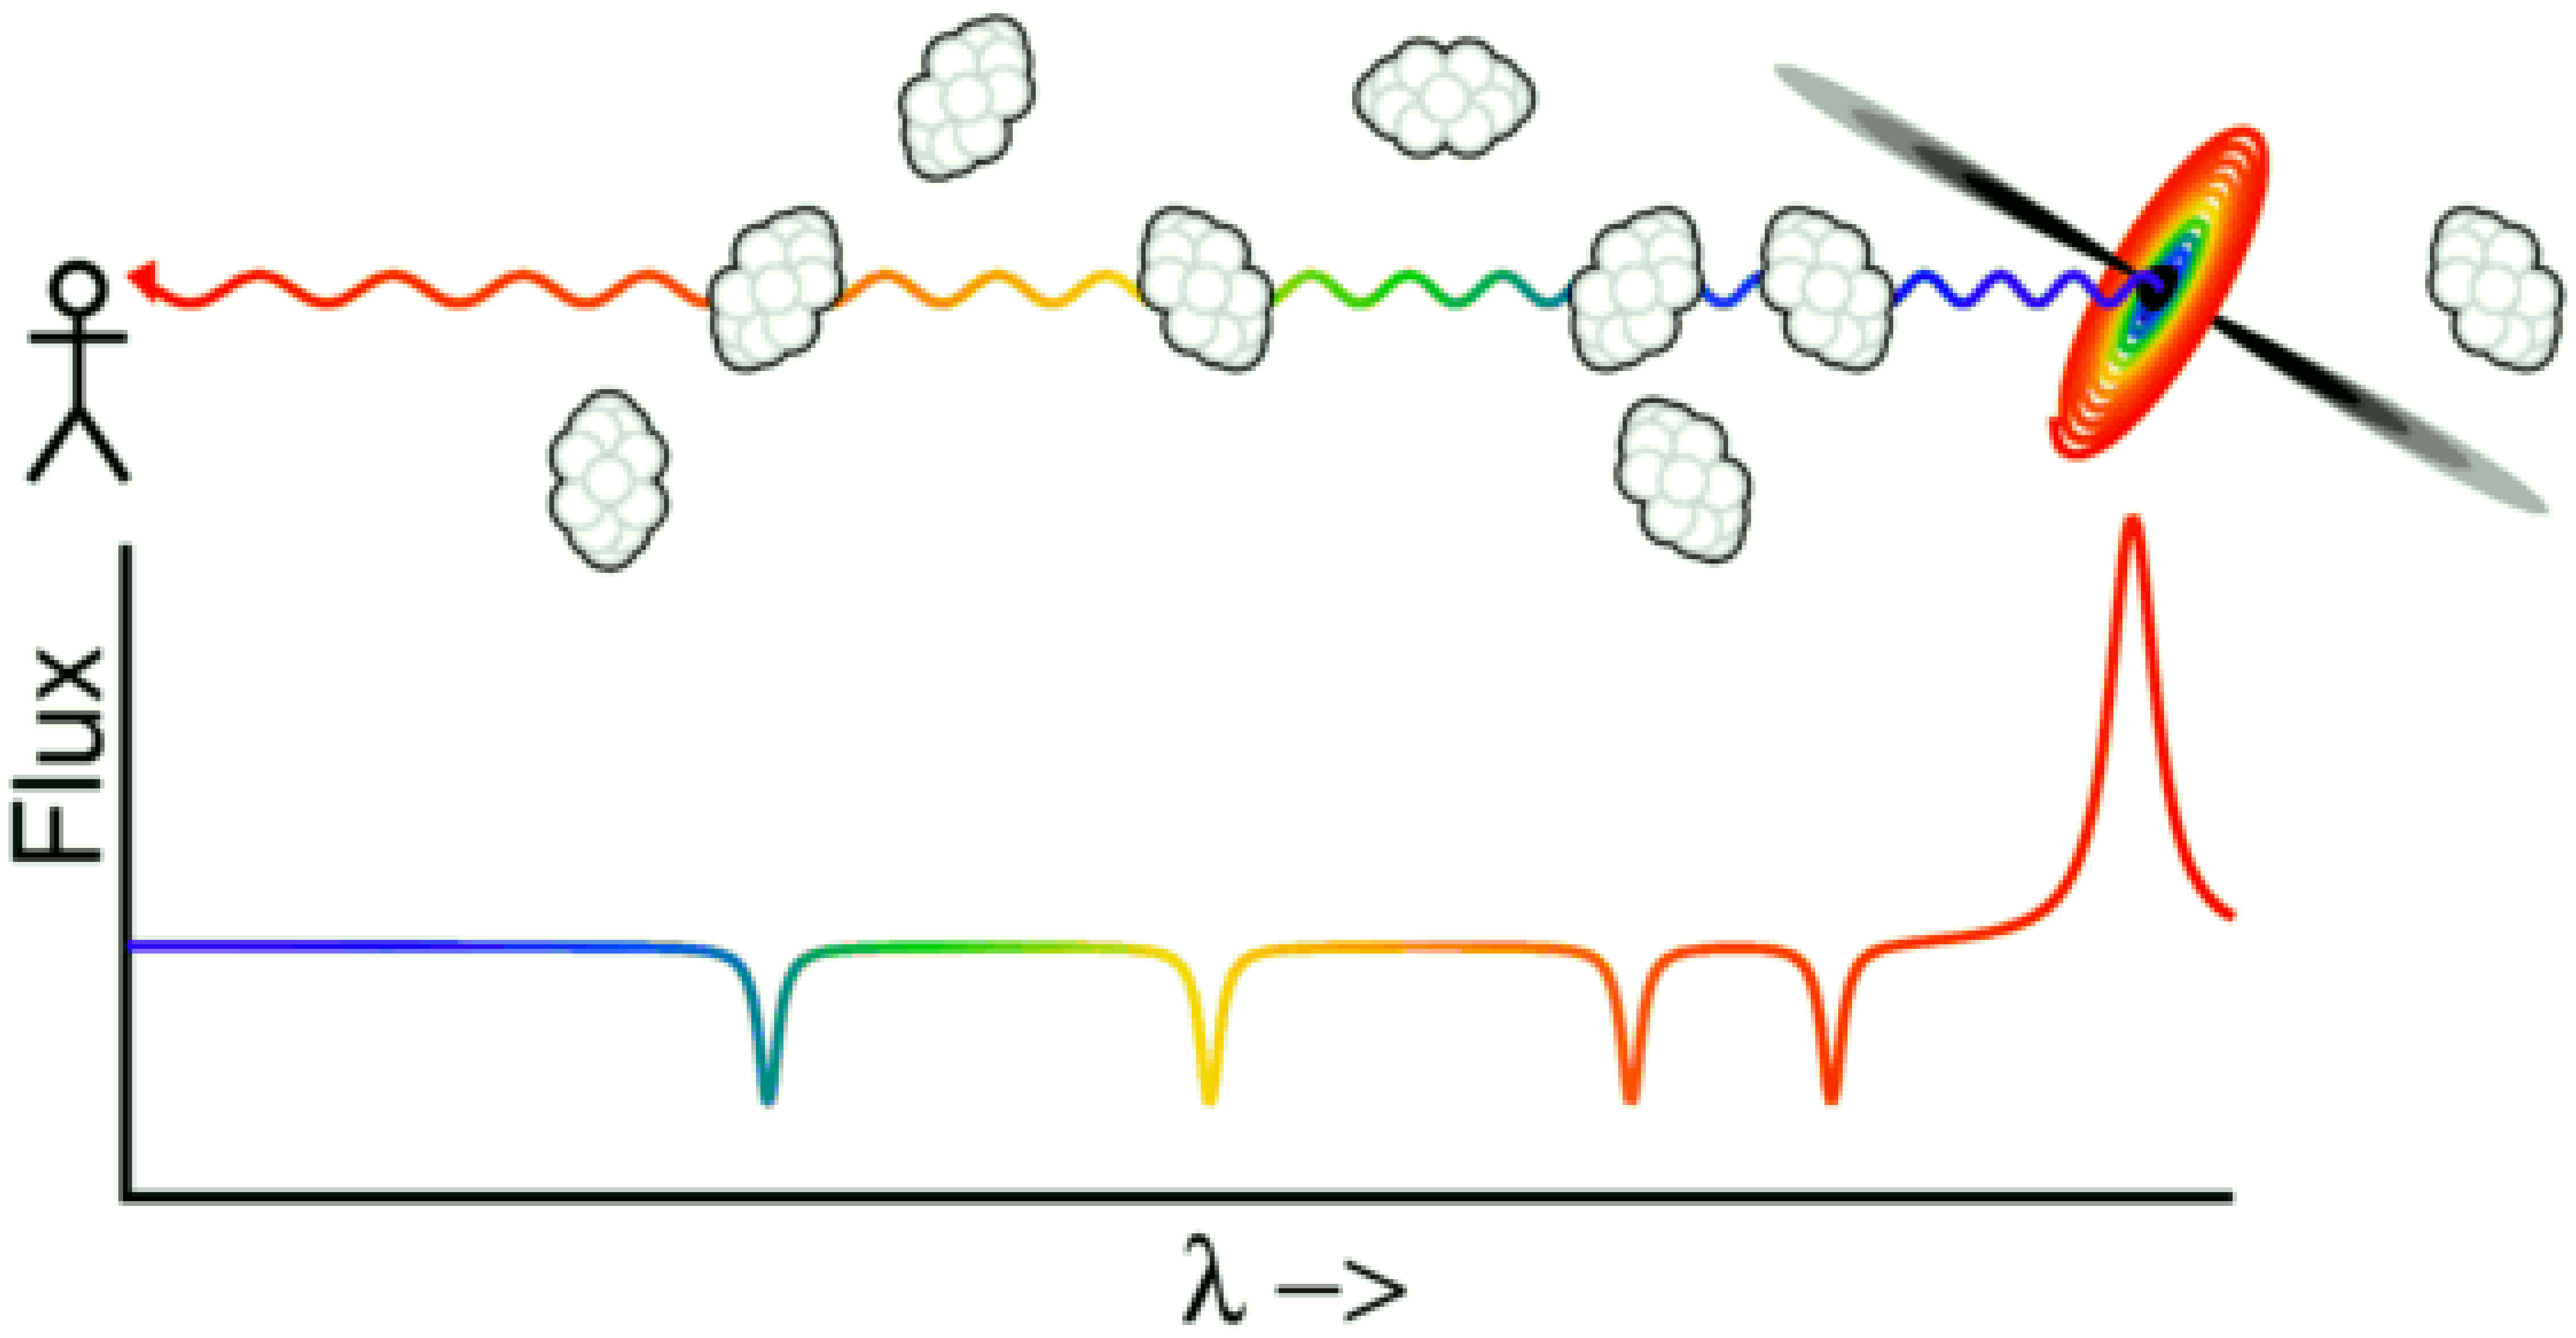
\includegraphics[width=12cm]{lyaf-75.eps}
  \caption{Illustration of the basic physics behind the \lya\ forest and how gas at different locations along the line of sight results in absorption lines at different wavelengths. (Image from {\tt http://www.astro.ucla.edu/})}
  \label{fig:LyaCartoon}
\end{figure}

The same logical progression also applies to the other lines in the Lyman-series, with the difference that lines deeper in the series have a smaller cross section for absorption. Therefore, you could imagine observing a \lyb\ and Ly\ $\gamma$\ forest at smaller wavelengths. Another important difference here, though, is that photons emitted from a background source with energies larger than \lyb\ will redshift through the \lyb\ wavelength and \textit{also} possibly through the \lya\ wavelength before reaching us. The photon's physical location when it redshifts through those two wavelengths will be completely different and, therefore, when observing absorption lines in the \lyb\ forest, it can be difficult to tell if the photons were absorbed by distant gas undergoing a \lyb\ transmission or closer gas undergoing a \lya\ transition. This problem is clearly exacerbated when considering higher-order lines since a larger number of distinct regions along the line of sight can contribute to the absorption.


We show two example quasar spectra in Figure \ref{fig:LyaExample}. The spectrum in the top panel is for a quasar at relatively low redshift and shows very little absorption. Meanwhile, the quasar in the bottom panel shows little absorption for emitted wavelengths redward of \lya\ but is heavily punctuated by absorption blueward of \lya\ due to intervening neutral hydrogen. It is this pattern of absorption features with $\lambda_{\beta} \leq \lambda_{\text{emitted}} \leq \lambda_{\alpha}$ that is referred to as the \lya\ forest.
 
\begin{figure}[h]
  \centering
  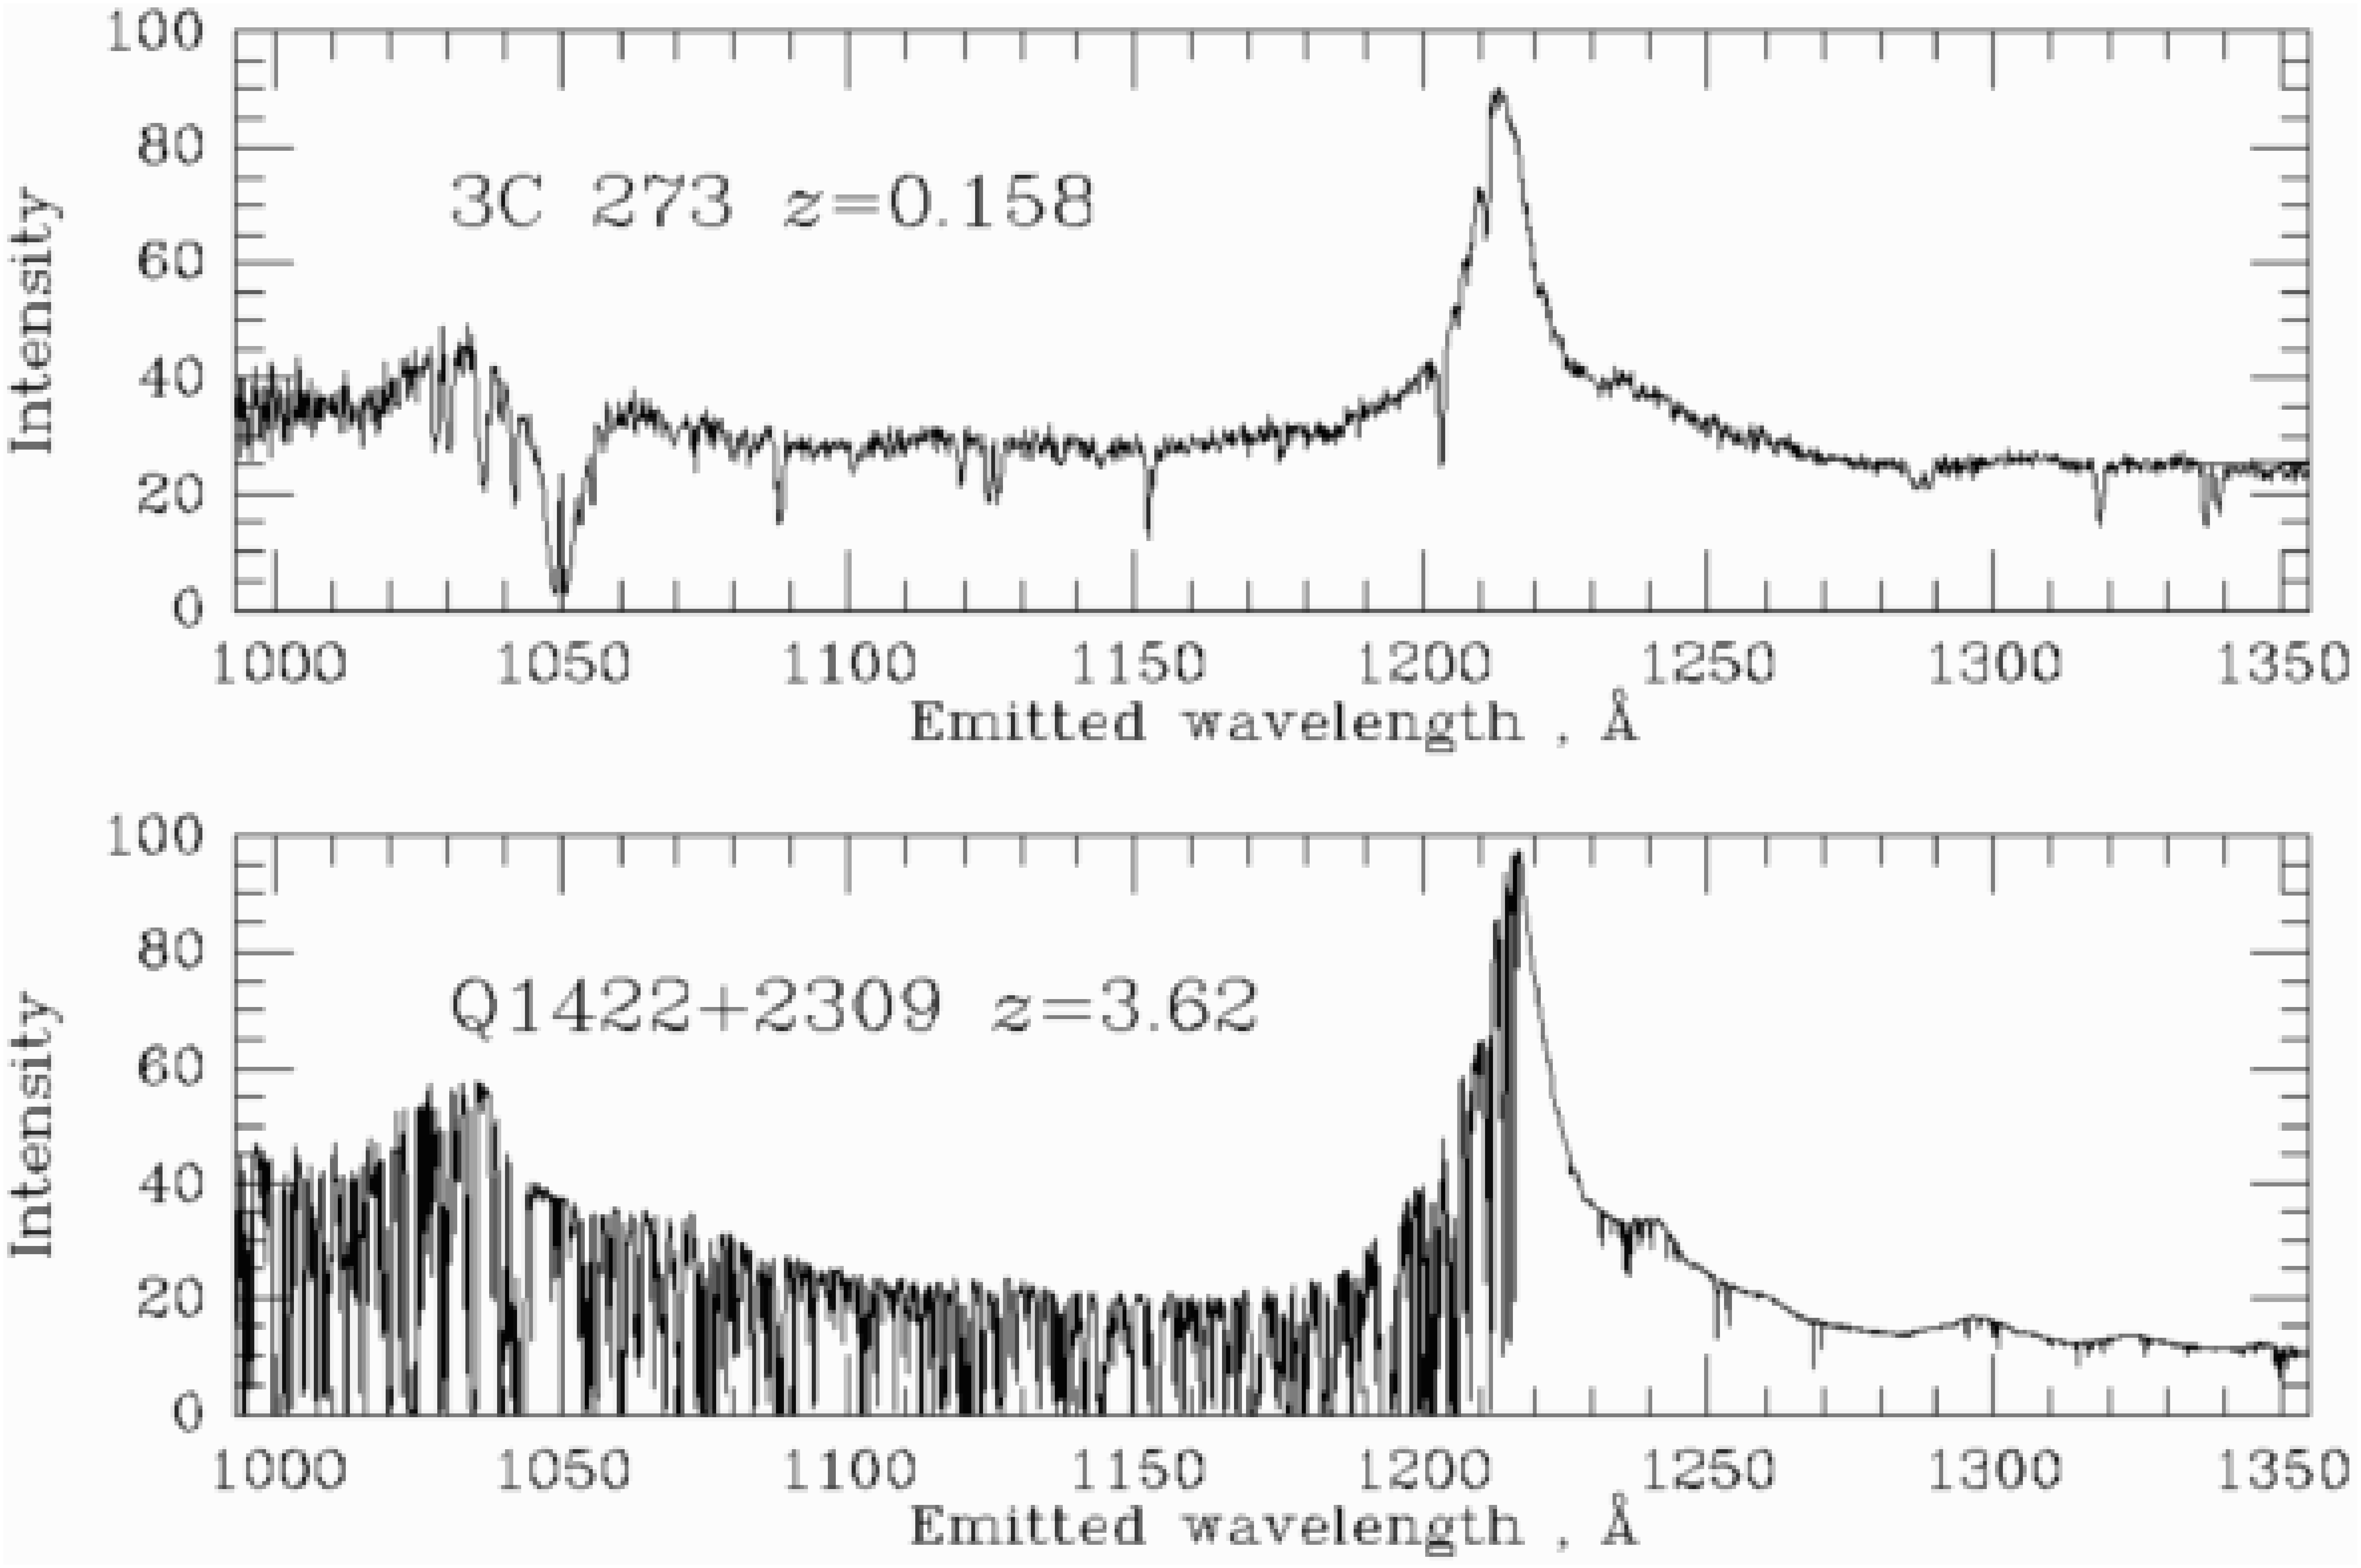
\includegraphics[width=12cm]{Lya-forest-60.eps}
  \caption{Flux as a function of rest-frame wavelength for a quasar at $z = 0.158$ (top) and $z = 3.62$ (bottom). The denser IGM at higher $z$ results in a dense ``forest" of absorption lines redward of the rest-frame \lya\ line in the lower panel. (Image from {\tt http://www.astro.ucla.edu/})}
  \label{fig:LyaExample}
\end{figure}

At this point, the \lya\ forest should sound like a perfect tool: if we want to map the distribution of neutral hydrogen along the line of sight to a distant bright source, we can simply map each absorption line in the \lya\ forest to a parcel of neutral hydrogen. However, the story becomes complicated here due to the extremely large cross section for \lya\ absorption. Namely, the optical depth\nomenclature[Zp]{Optical Depth}{Optical depth, denoted by $\tau$, is a quantity that describes that likelihood for a photon to be absorbed, usually by a gas. The fraction of photons that will pass through the gas unabsorbed is $e^{-\tau}$.} for \lya\ absorption of a neutral hydrogen gas parcel obeys the relationship

\begin{align}
\tau_{\alpha} &\approx 3.3 \times 10^{4} \xhi (1 + \delta) \left[\dfrac{1+z}{6.5}\right]^{3/2}.
\end{align}

Using this expression, we can calculate the minimum neutral fraction needed for a gas parcel at mean density to allow 1\% transmission at $z = 5.5$:

\begin{align}
.01 &= e^{-\tau_{\text{min}}} \implies \tau_{\text{min}} \approx 4.6\\
4.6 &\approx \tau_{\alpha} x_{\text{HI,min}} \\
\implies x_{\text{HI,min}} &\approx 0.00014.
\end{align}


This reveals the fly in the ointment here: even a gas parcel that is 99.9\% ionized will allow less than 1\% transmission at the redshifts of interest for reionization. This allows absorption features to be caused by highly-ionized gas that happens to be over-dense. Therefore, we can not simply map absorption lines in the \lya\ forest to regions of significantly-neutral hydrogen. In fact, the second example quasar we see in Figure \ref{fig:LyaExample} shows significant \lya\ absorption and is located at $z = 3.62$, \textit{much later than the end of reionization}. At this point, the reader may ask what utility does the \lya\ forest have at all? Well, an enormous amount. To name a very few applications outside of reionization, since \lya\ absorption can be caused by matter overdensities the \lya\ forest can be used to measure the matter power spectrum in the IGM which in turn can be used to measure the baryon acoustic oscillations (BAO), provide lower limits on the mass of the dark matter (\citealt{Viel:2013fqw}), and constrain dark energy. Additionally, absorption features due to damped \lya\ absorbers (DLAs) can be used to measure the primordial deuterium abundance as a test of big bang nucleosynthesis.\\
\textcolor{white}{suspense!}\\
\noindent But how to constrain the EoR?



\subsubsection{Evolution of $\tau_{\text{eff}}$}

% The Gunn-Peterson optical depth to \lya\ photons is \tau_{\text{GP}} = \dfrac{\pi e^2}{m_e c} f_{\alpha} \lambda_{\alpha} H^{-1}(z)n_{\text{HI}}

% Absorption is understood as being caused by the fluctuating Gunn-Peterson effect, low density regions in approximate thermal equilibrium between photoionization heating by the UV background and adiabatic cooling due to the Hubble expansion, rather than discrete \lya\ absorbers.

% By studying the evolution of the average transmitted flux or effective optical depth, one can trace the evolution in the 

% You probably want to re-read and refer to Lidz et al. that discuss that the evolution in the effective optical depth can be replicated by density fluctuations

A common assumption made in analyzing quasar spectra at $z < 6$ is that, due to the presence of transmission in the spectra, the IGM must already be highly-ionized. 



\subsubsection{Dark Pixel Covering Fraction}
\subsubsection{Dark Gap Sizes}
\subsubsection{Damping Wing Redward of \lya}

\begin{figure}[h]
  \centering
  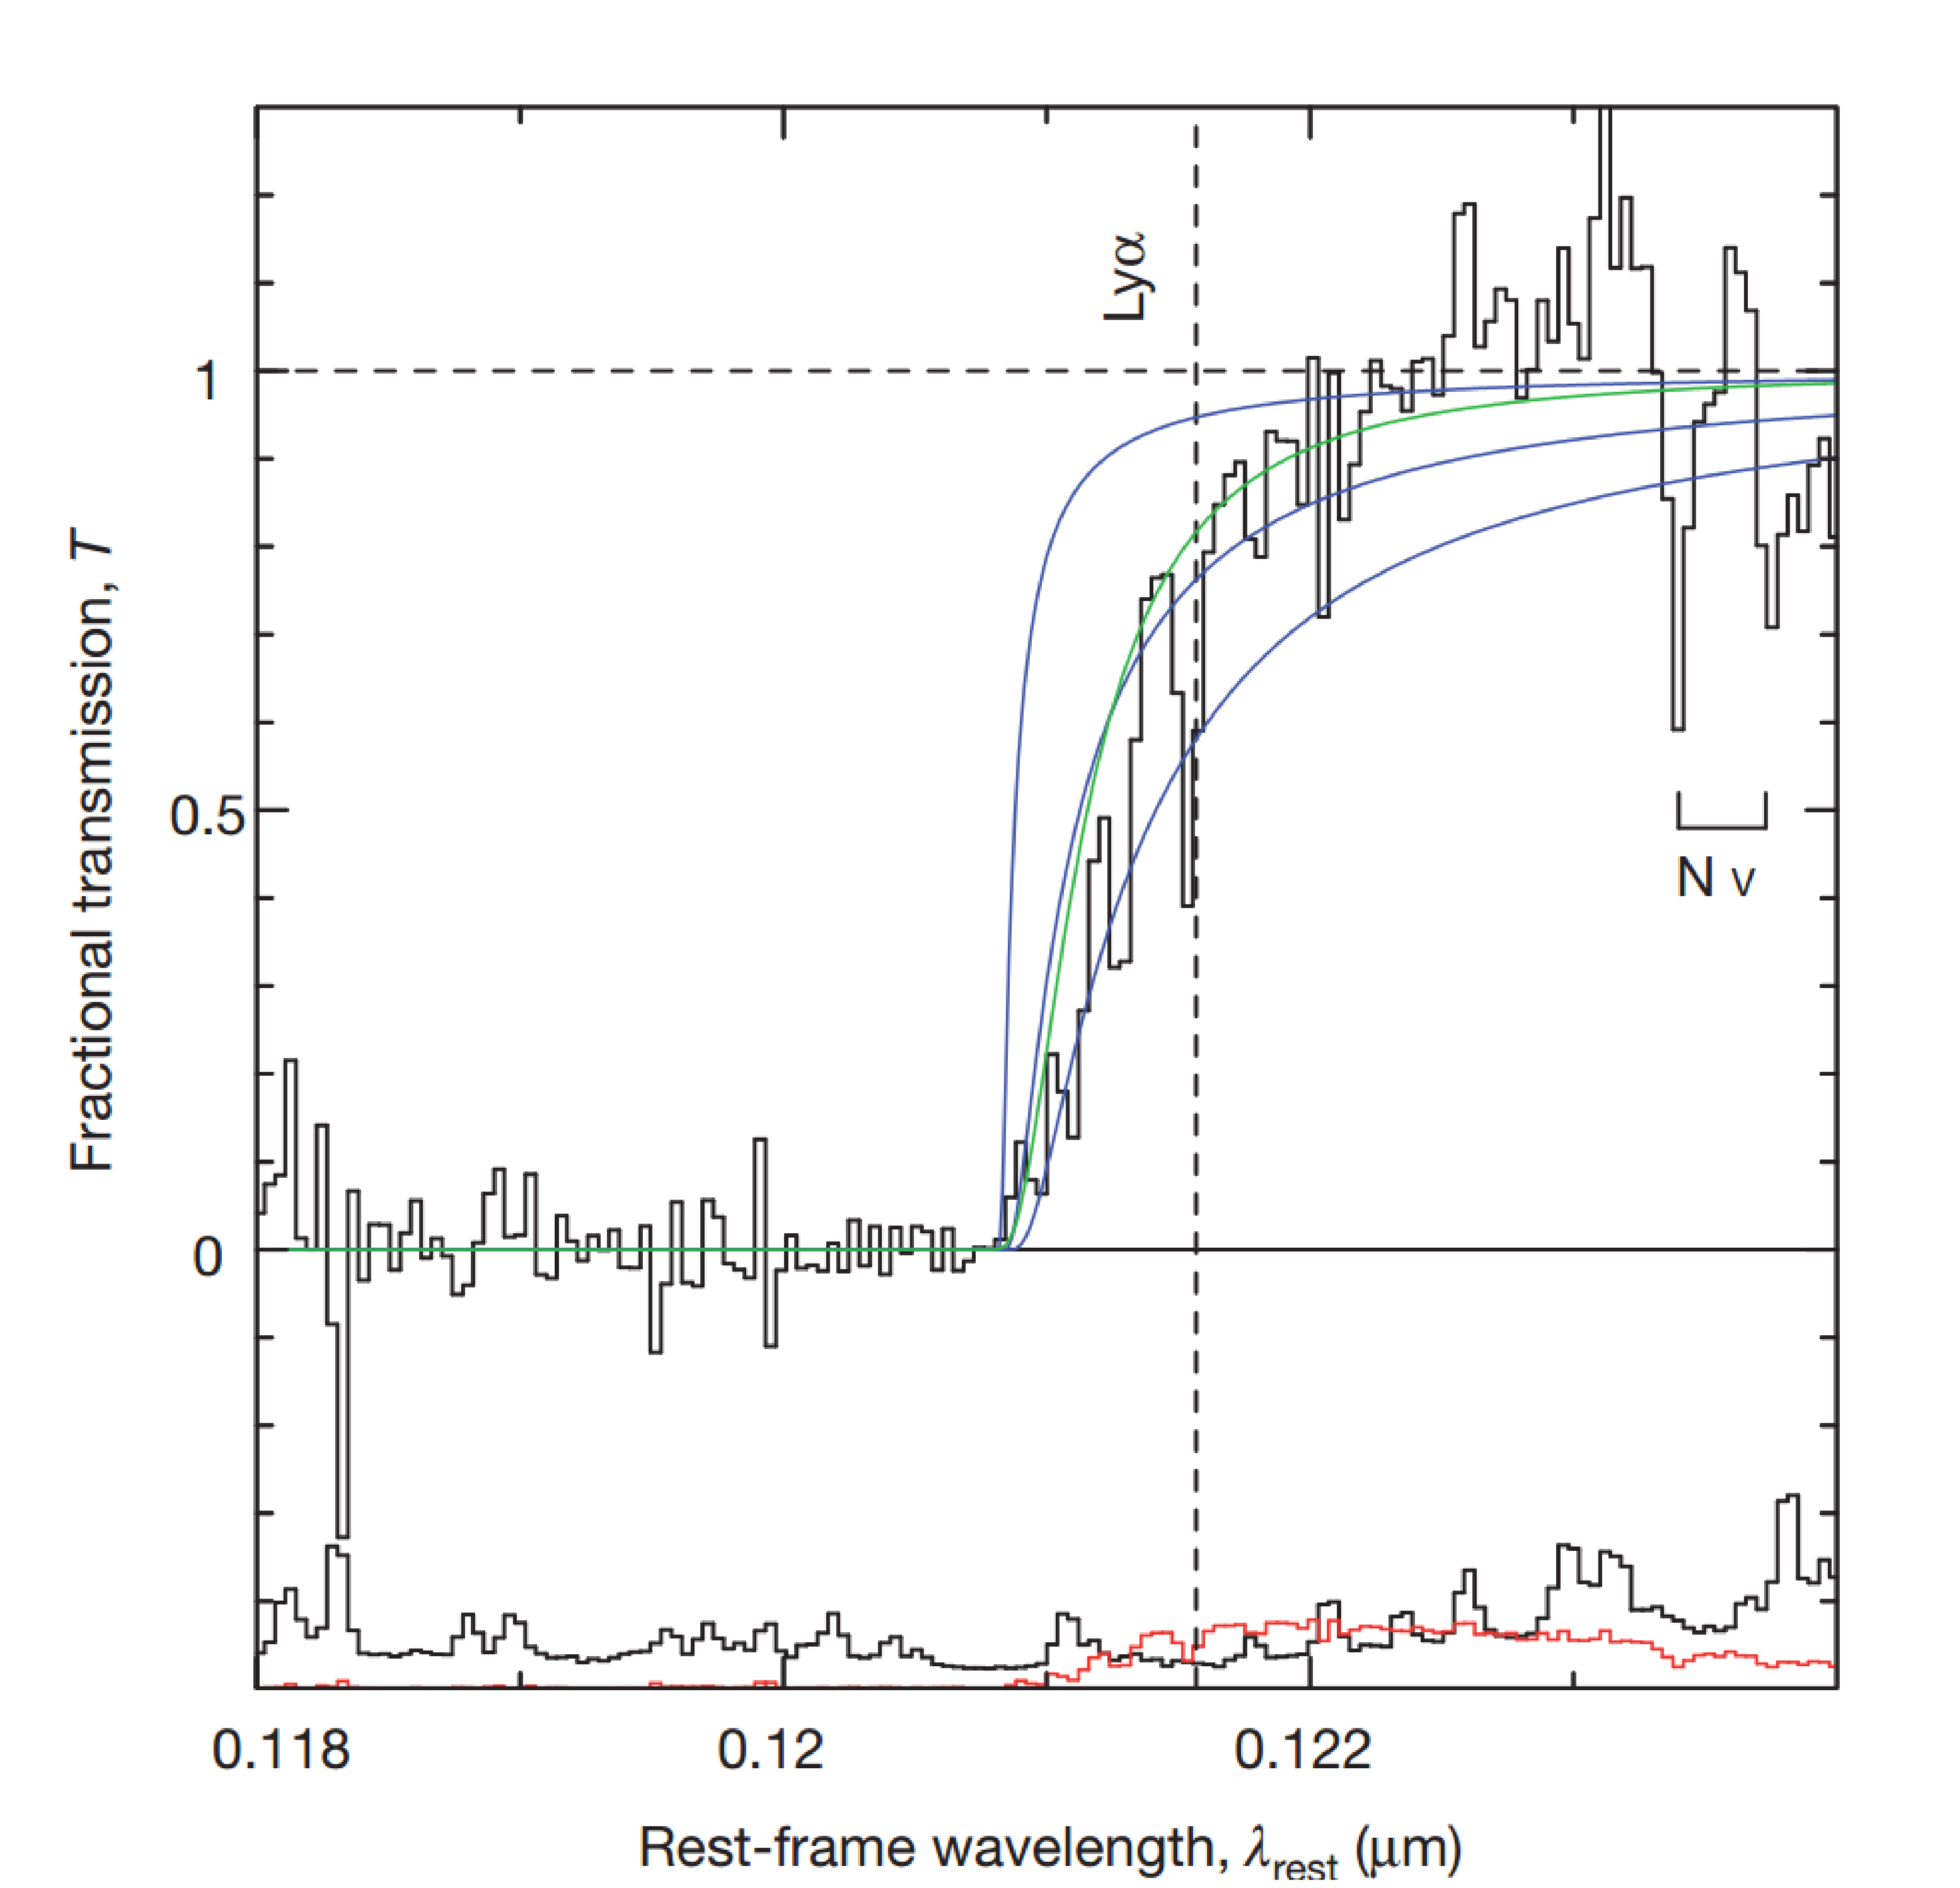
\includegraphics[width=8cm]{z7p085_DampingWing.eps}
  \caption{Quasar ULAS J1120+0641 identified at redshift $z = 7.085$ along with several fits for the damping wing.}
  \label{fig:Chornock}
\end{figure}



\subsection{The 21-cm Line}
\subsection{The Cosmic Microwave Background}
\subsection{\lya Emitters}
\subsection{Luminosity Function Measurements}

\section{Current Constraints on the Timing and Nature of the EoR}

\begin{enumerate}
\item Bouwens et al. (2015) might be good to include here. Strengthens argument that galaxies reionized the Universe and that quasars/AGN did not.
\end{enumerate}
% ----------------------------------------------------------------------



